\documentclass[a4paper]{article}
\usepackage[utf8]{inputenc}
\usepackage[spanish, es-tabla, es-noshorthands]{babel}
\usepackage[table,xcdraw]{xcolor}
\usepackage[a4paper, footnotesep = 1cm, width=20cm, top=2.5cm, height=25cm, textwidth=18cm, textheight=25cm]{geometry}
%\geometry{showframe}

\usepackage{tikz}
\usepackage{amsmath}
\usepackage{amsfonts}
\usepackage{amssymb}
\usepackage{float}
\usepackage{graphicx}
\usepackage{caption}
\usepackage{subcaption}
\usepackage{multicol}
\usepackage{multirow}
\setlength{\doublerulesep}{\arrayrulewidth}
\usepackage{booktabs}

\usepackage{hyperref}
\hypersetup{
    colorlinks=true,
    linkcolor=blue,
    filecolor=magenta,      
    urlcolor=blue,
    citecolor=blue,    
}

\newcommand{\quotes}[1]{``#1''}
\usepackage{array}
\newcolumntype{C}[1]{>{\centering\let\newline\\\arraybackslash\hspace{0pt}}m{#1}}
\usepackage[american]{circuitikz}
\usetikzlibrary{calc}
\usepackage{fancyhdr}
\usepackage{units} 

\graphicspath{{../Ejercicio-1/}{../Ejercicio-2/}{../Ejercicio-3/}{../Ejercicio-4/}}

\pagestyle{fancy}
\fancyhf{}
\lhead{22.01 Teoría de Circuitos}
\rhead{Mechoulam, Lambertucci, Rodriguez Turco, Londero, Galdeman}
\rfoot{\centering \thepage}

\begin{document}

%%%%%%%%%%%%%%%%%%%%%%%%%
%		Caratula		%
%%%%%%%%%%%%%%%%%%%%%%%%%

\begin{titlepage}
\newcommand{\HRule}{\rule{\linewidth}{0.5mm}}
\center
\mbox{\textsc{\LARGE \bfseries {Instituto Tecnológico de Buenos Aires}}}\\[1.5cm]
\textsc{\Large 22.01 Teoría de Circuitos}\\[0.5cm]


\HRule \\[0.6cm]
{ \Huge \bfseries Trabajo práctico N$^{\circ}$5}\\[0.4cm] 
\HRule \\[1.5cm]


{\large

\emph{Grupo 3}\\
\vspace{3px}

\begin{tabular}{lr} 	
\textsc{Mechoulam}, Alan  &  58438\\
\textsc{Lambertucci}, Guido Enrique  & 58009 \\
\textsc{Rodriguez Turco}, Martín Sebastian  & 56629 \\
\textsc{Londero Bonaparte}, Tomás Guillermo  & 58150 \\
\textsc{Galdeman}, Agustín & 59827\\
\end{tabular}

\vspace{20px}

\emph{Profesores}\\
Jacoby, Daniel Andrés\\
Belaustegui Goitia, Carlos\\
Iribarren, Rodrigo Iñaki\\
\vspace{3px}
%\textsc{} \\	

\vspace{100px}

\begin{tabular}{ll}

Presentado: & */*/19\\

\end{tabular}

}

\vfill

\end{titlepage}


%%%%%%%%%%%%%%%%%%%%%
%		Indice		%
%%%%%%%%%%%%%%%%%%%%%

\tableofcontents
\newpage

%%%%%%%%%%%%%%%%%%%%%
%		Informe		%
%%%%%%%%%%%%%%%%%%%%%
\section{Aproximacion de Chebycheff con celda Rauch}
	\documentclass[a4paper]{article}
\usepackage[utf8]{inputenc}
\usepackage[spanish, es-tabla, es-noshorthands]{babel}
\usepackage[table,xcdraw]{xcolor}
\usepackage[a4paper, footnotesep = 1cm, width=20cm, top=2.5cm, height=25cm, textwidth=18cm, textheight=25cm]{geometry}
%\geometry{showframe}

\usepackage{tikz}
\usepackage{amsmath}
\usepackage{amsfonts}
\usepackage{amssymb}
\usepackage{float}
\usepackage{graphicx}
\usepackage{caption}
\usepackage{subcaption}
\usepackage{multicol}
\usepackage{multirow}
\setlength{\doublerulesep}{\arrayrulewidth}
\usepackage{booktabs}

\usepackage{hyperref}
\hypersetup{
    colorlinks=true,
    linkcolor=blue,
    filecolor=magenta,      
    urlcolor=blue,
    citecolor=blue,    
}

\newcommand{\quotes}[1]{``#1''}
\usepackage{array}
\newcolumntype{C}[1]{>{\centering\let\newline\\\arraybackslash\hspace{0pt}}m{#1}}
\usepackage[american]{circuitikz}
\usetikzlibrary{calc}
\usepackage{fancyhdr}
\usepackage{units} 

\graphicspath{{../Ejercicio-1/}{../Ejercicio-2/}{../Ejercicio-3/}{../Ejercicio-4/}}

\pagestyle{fancy}
\fancyhf{}
\lhead{22.01 Teoría de Circuitos}
\rhead{Mechoulam, Lambertucci, Rodriguez Turco, Londero, Galdeman}
\rfoot{\centering \thepage}
\begin{document}

\subsection{Introducción}

En esta sección se implementó un filtro Band-Pass utilizando una aproximación \textbf{Chebycheff} e implementandola con celdas \textbf{Rauch}, el filtro a diseñar deberá cumplir con la siguiente plantilla.
\begin{table}[H]
\centering
\begin{tabular}{|c|c|}
\hline
$Pendiente$      & -40$\frac{dB}{dec}$           \\ \hline
$f_p$      & 28kHz          \\ \hline
$B$      & $\frac{1}{10}$           \\ \hline
$A_p$      & 3dB               \\ \hline
$Filtro$      & BP              \\ \hline
$|Z_{in}|$ & $\geq 50k \Omega$ \\ \hline
\end{tabular}
\end{table}
\subsection{Aproximación de Chebycheff.}
Para esta sección se utlizó la aproximación de \textbf{Chebyfeff}, además se propuso una plantilla mas restrictiva, con el fin de asegurar el cumplimiento de la original. 

Se despejó el valor de $f_p^+$ y $f_p^-$ 
\begin{align}
f_0^2 = f_p^+ \cdot f_p^- \\
B = \frac{\Delta f_p}{f_0}\\
f_p^+ =29.435 kHz  \ \ \ f_p^- = 26.635 kHz
\end{align}
Luego teniendo en cuenta que la pendiente originalmente es de 40dB por decada se tomo la frecuencia de atenuación acorde  talque mantenga las condiciones de simetría, siendo estas: $f_a^+= 294.35kHz y f_a^- = 2.635kHz$.


Siendo esta la plantilla final.
\begin{table}[H]
\centering
\begin{tabular}{|c|c|}
\hline
$f_s^-$      & 2.6635 kHz          \\ \hline
$f_p^-$      & 26.635 kHz         \\ \hline
$f_p^+$      & 29.435 kHz           \\ \hline
$f_s^+$      & 294.35 kHz          \\ \hline
$A_s$      & 40dB           \\ \hline
$A_p$      & 1dB               \\ \hline
\end{tabular}
\end{table}
Obteniendo la siguiente función transferencia:
\begin{align}
	H(s)=\frac{s}{\left( \frac{s}{23728.54}\right) ^2+s\cdot \frac{23728.54}{3.23}+1}\cdot \frac{s}{\left( \frac{s}{33052.25} \right)^2+s\cdot \frac{33052.25}{3.23}+1}
\end{align}
al cual le corresponde la siguiente respues en frecuencia:

Y el siguiente diagrama de polos y ceros:
\begin{figure}[H]
	\centering
	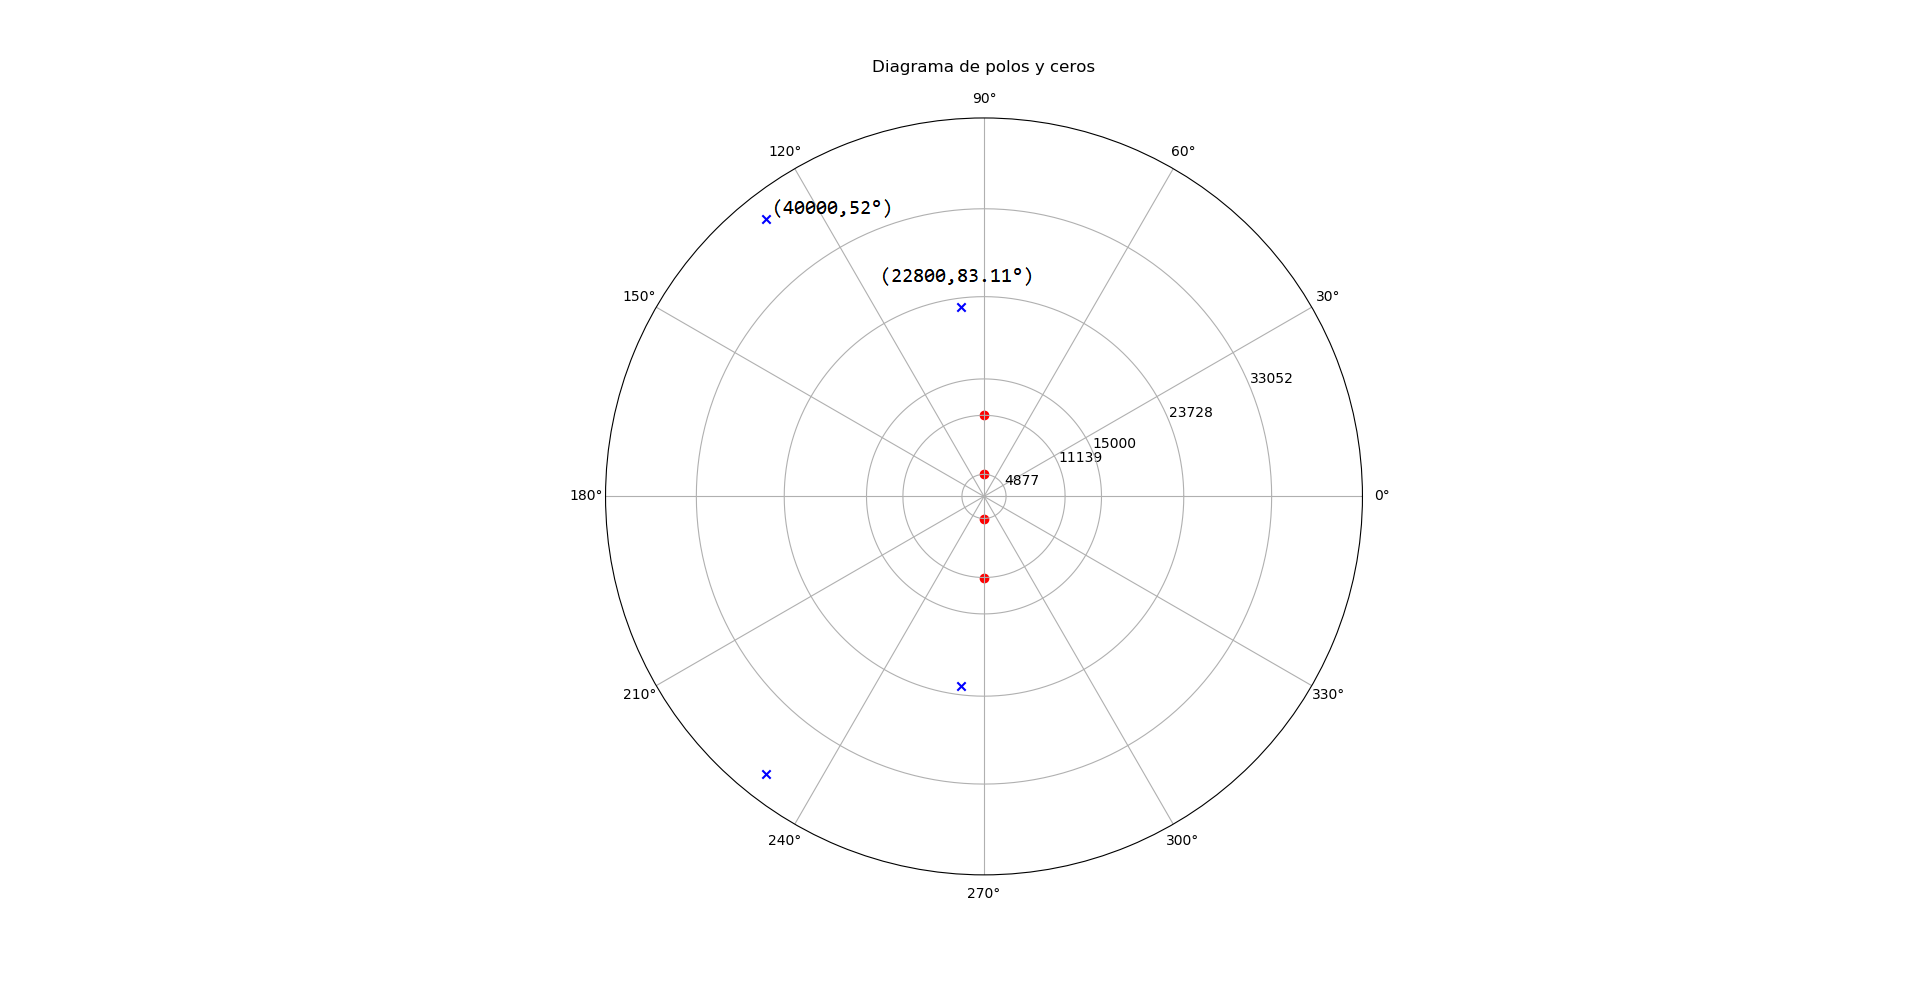
\includegraphics[width=0.5\textwidth]{Imagenes-Ej2/DiagramaPolosYCeros.png}
	\label{fig:stepresponse}
	\caption{Diagrama Polos y Ceros}
\end{figure}

Teniendo los pares de polos conjugados un Q de 3.23	


\subsubsection{Elecciones de diseño}
Se decidió armar etapas con celdas segundo orden en cascada dado a que el orden es 4.
Para la asociación de polos se tomo criterio agrupar cada par de polos con 1 cero , agrupandolos de las siguiente forma.
\begin{figure}[H]
	\centering
	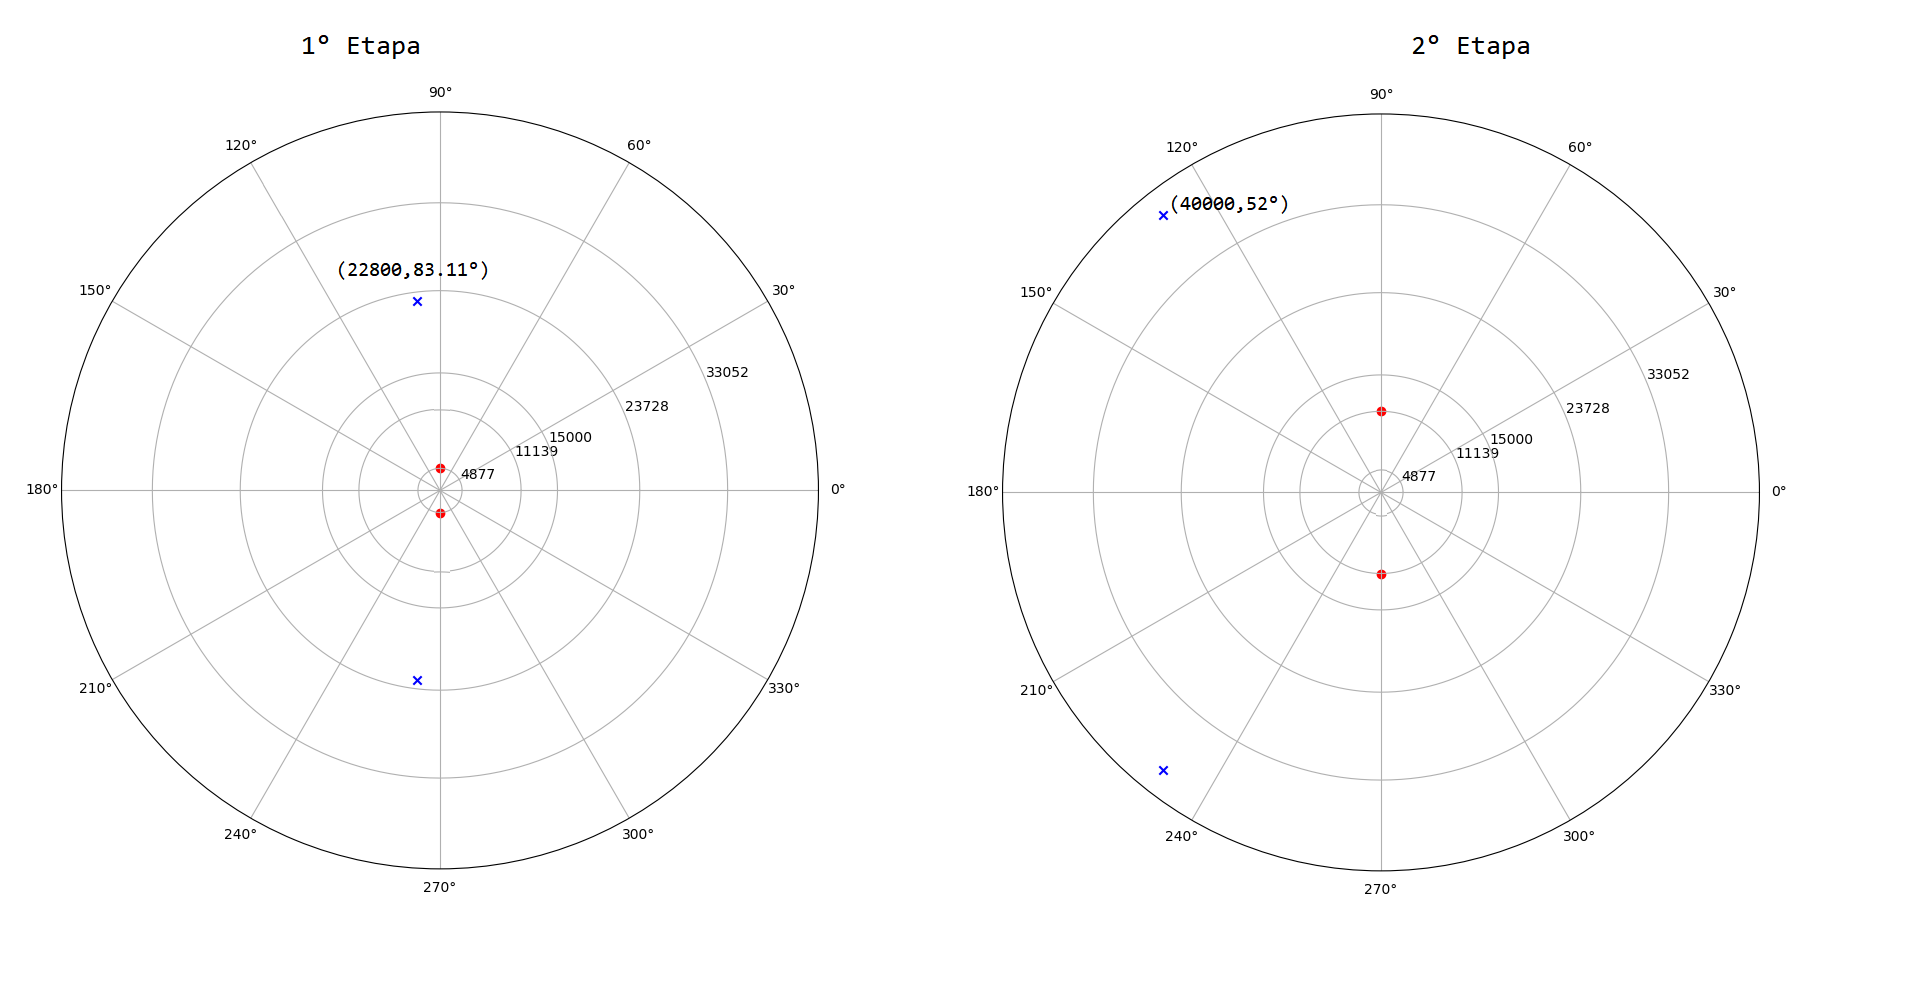
\includegraphics[width=\textwidth]{Imagenes-Ej2/UnionCeros.png}
	\label{fig:CeroPoleUnion}
	\caption{Diagrama Polos y Ceros para cada etapa}
\end{figure}

\subsection{Celda Rauch.}
La celda Rauch es una modificación de la celda Deliyannis-Friend incluyendo uan realimentación positiva.
\begin{figure}[H]
	\centering
	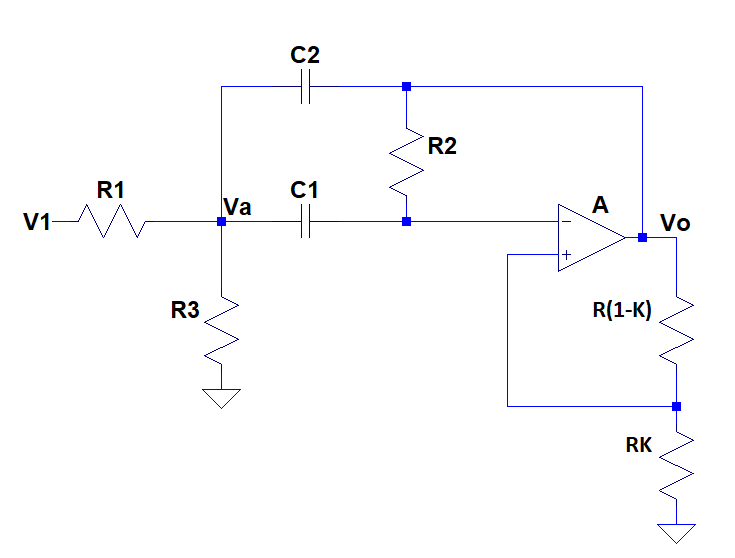
\includegraphics[width=0.5\textwidth]{Imagenes-Ej2/Circuit.PNG}
	\label{fig:graph}
	\caption{Circuito celda Rauch Band-Pass.}
\end{figure}
\subsubsection{Cálculo Analítico}
---
\subsubsection{Elecciones de diseño}

\begin{center}
	\huge{\textcolor{red}{\textbf{Tabla sensibilidades}}}
\end{center}
En base a esta tabla se tomo especial cuidado en la elección de componentes y en el matcheo de impedancias.

Los componentes utilizados fueron los siguientes:
\begin{table}[H]
\centering
\begin{tabular}{lllll}
\multicolumn{1}{c}{Componente} & \multicolumn{1}{c}{1er Etapa} & \multicolumn{1}{c}{Composición} & 2da Etapa      & Composición           \\ \hline
$R_1$                          & $7.3 k\Omega$                 & $10k // 27k  \Omega$            & $5.24 k\Omega$ & $5.6k // 82k  \Omega$ \\
$R_2$                          & $5.56 k\Omega$                & $5.6k // 680k  \Omega$          & $3.99 k\Omega$ & $82 + 3.9k  \Omega$   \\
$R_3$                          & $1.43 k\Omega$                & $1.5 k // 33k  \Omega$          & $1.03k\Omega$  & $27 + 1k  \Omega$     \\
$R_4$                          & $3.49 k\Omega$                & $3.9k // 33k  \Omega$           & $3.49 k\Omega$ & $3.9k // 33k  \Omega$ \\
$R_5$                          & $1 k\Omega$                   & $1 k  \Omega$                   & $1 k\Omega$    & $1 k\Omega$           \\
$C_1$                          & 2.2 nF                        & 2.2 nF                          & 2.2 nF         & 2.2 nF                \\
$C_2$                          & 2.2 nF                        & 2.2 nF                          & 2.2 nF         & 2.2 nF               
\end{tabular}
\end{table}

Se calculó el error porcentual asociado a la aproximación de la resistencias viendose en la siguiente tabla.
\begin{table}[H]
\centering
\begin{tabular}{lll}
\multicolumn{1}{c}{Error Porcentual} & \multicolumn{1}{c}{1er Etapa} & \multicolumn{1}{c}{2da Etapa} \\ \hline
$R_1$                                & 0.1 $\%$                      & $0.038  \%$                   \\
$R_2$                                & 0.1 $\%$                      & 0.2 $\%$                      \\
$R_3$                                & 0.4 $\%$                      & 0.1 $\%$                      \\
$R_4$                                & 0.1 $\%$                      & 0.1 $\%$                      \\
$R_5$                                & $\approx 0 \%$                & $\approx 0 \%$                \\
$C_1$                                & $\approx 0 \%$                & $\approx 0 \%$                \\
$C_1$                                & $\approx 0 \%$                & $\approx 0 \%$               
\end{tabular}
\end{table}

Cabe destacar que todas las imepdancias que fueron colocadas en el circuito fueron elegidas entre varias de su mismo tipo, con la finalidad de poner impedancias que sean realmente de los valores deseados.

\subsubsection{Acoplamiento de Impedancias.}

Para que ambas etapas no se carguen entre si la impedancia de entrada de la segunda etapa debe ser mucho mayor a la de salida de la primera, para lo siguiente se obtuvieron las impedancias de entrada de ambas celdas, incluyendo la de salida de la primera.
\begin{figure}[H]
	\centering
	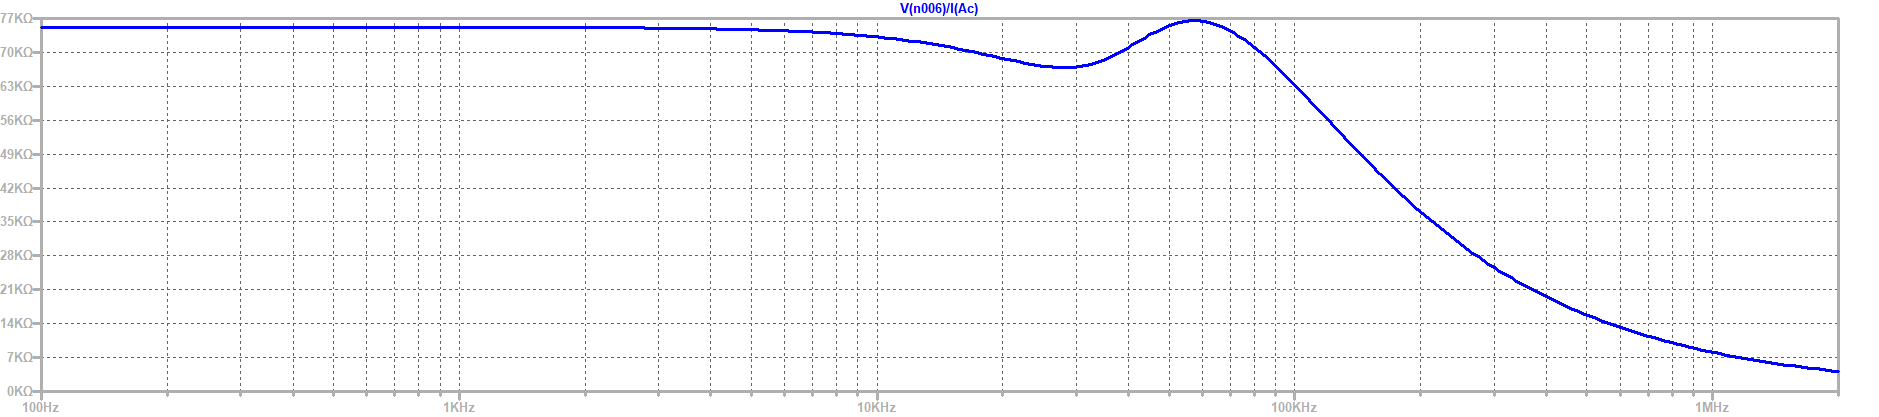
\includegraphics[width=\textwidth]{Imagenes-Ej2/ZinE1.png}
	\label{fig:graph}
	\caption{Impedancia de entrada 1er etapa.}
\end{figure}

\begin{figure}[H]
	\centering
	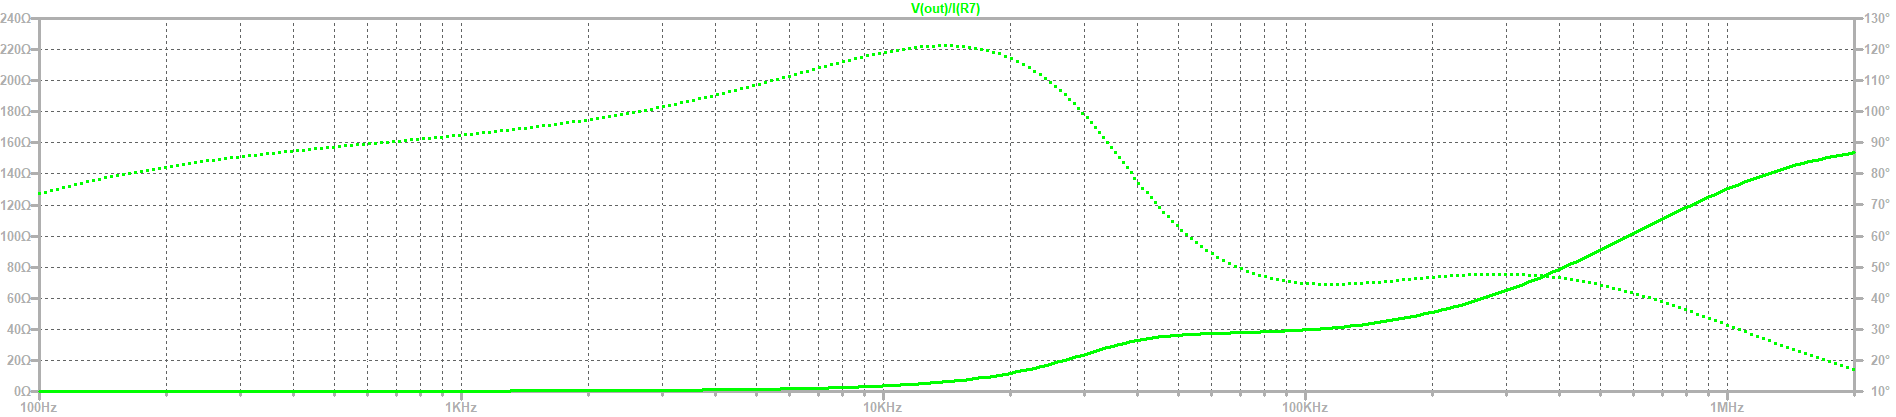
\includegraphics[width=\textwidth]{Imagenes-Ej2/ZoutE1.png}
	\label{fig:graph}
	\caption{Impedancia de salida 1er etapa.}
\end{figure}


\begin{figure}[H]
	\centering
	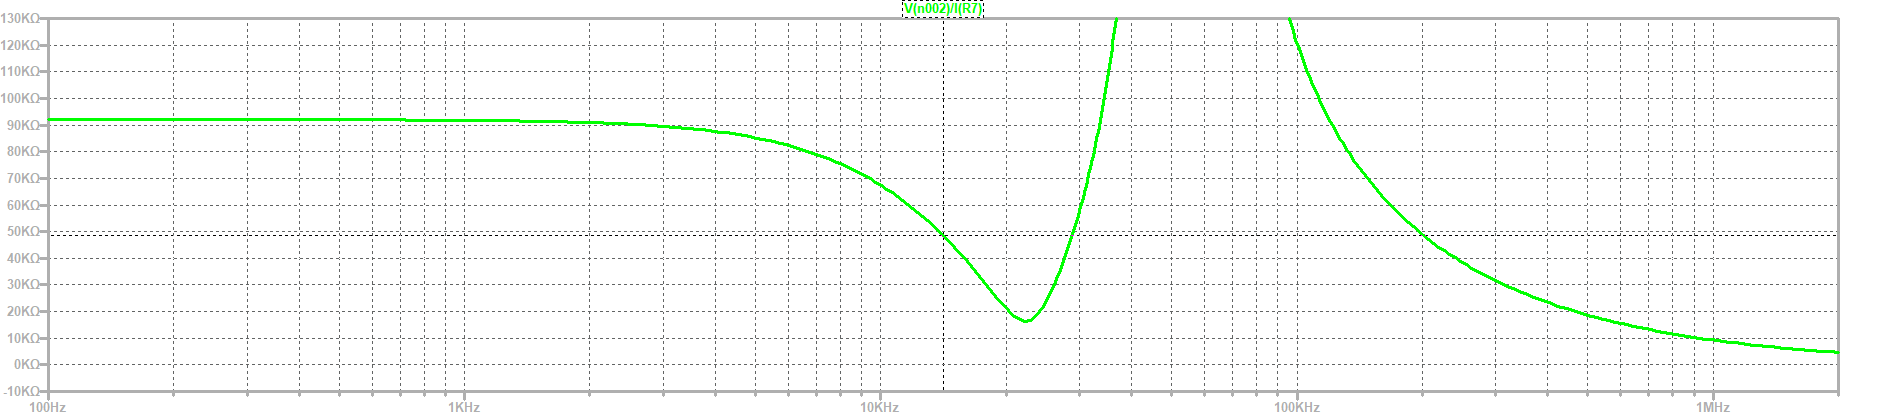
\includegraphics[width=\textwidth]{Imagenes-Ej2/ZinE2.png}
	\label{fig:graph}
	\caption{Impedancia de entrada 2da etapa.}
\end{figure}

\subsection{Respuesta en Frecuencia.}
Se realizó un análisis de Montecarlo a la respuesta en frecuencia del circuito, utilizando una tolerancia de las resistencias al 1$\%$ y capacitores al 10$\%$ obteniendo la siguiente disperción.
%\begin{figure}[H]
%	\centering
%	\includegraphics[width=0.4\textwidth]{/ImagenesEjercicio3/Graph.png}
%	\label{fig:graph}
%\end{figure}
También se midió la respuesta en frecuencia del filtro y se cotejó con la simulación.
\begin{figure}[H]
	\centering
	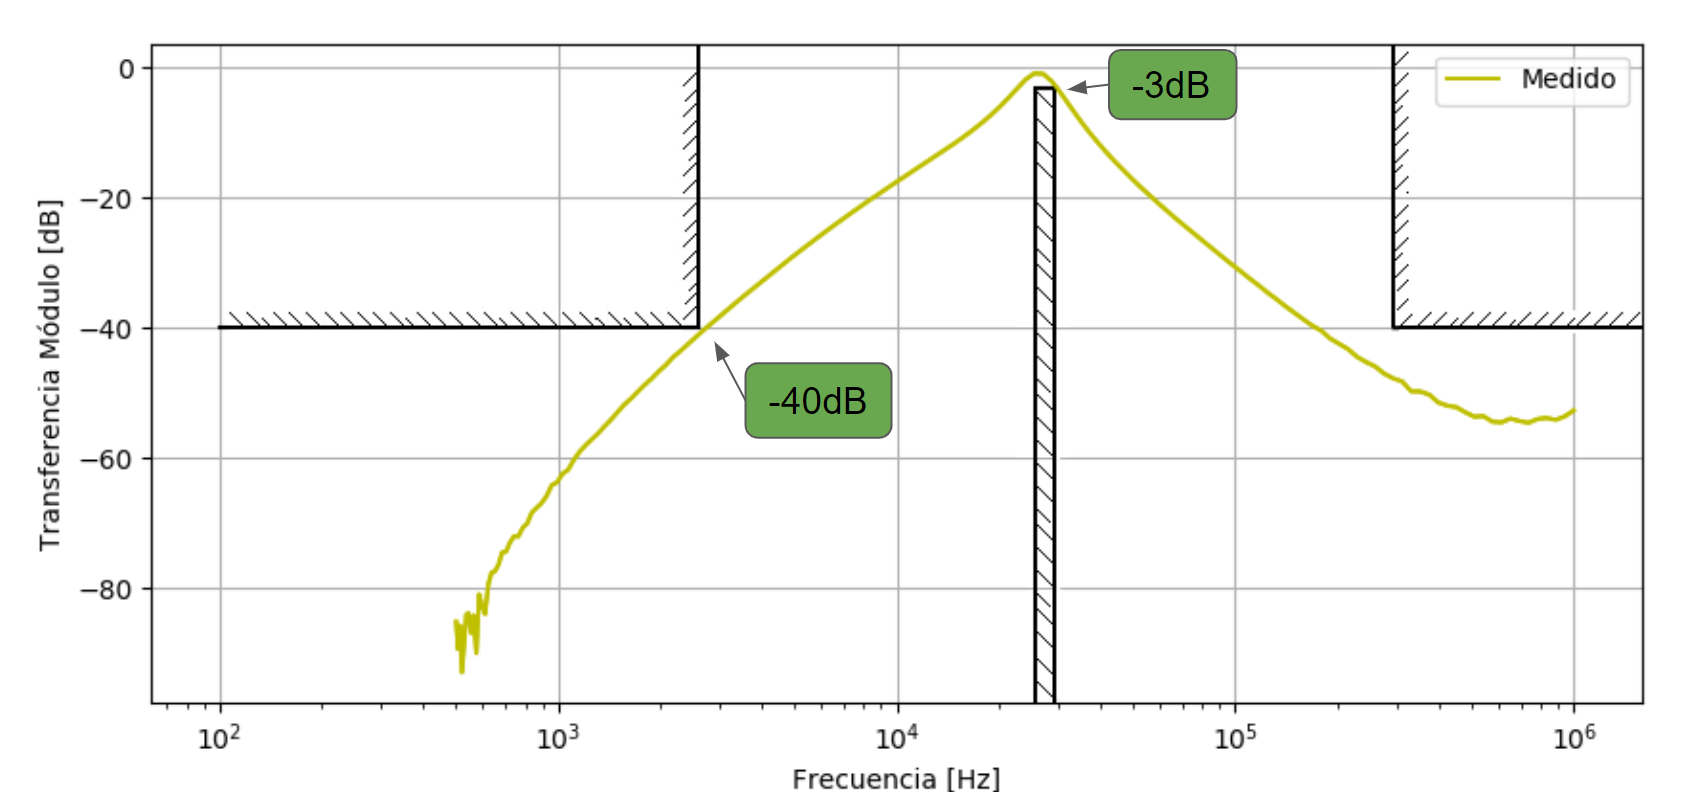
\includegraphics[width=\textwidth]{Imagenes-Ej2/BodeRauch.png}
	\label{fig:graph}
\end{figure}
\begin{figure}[H]
	\centering
	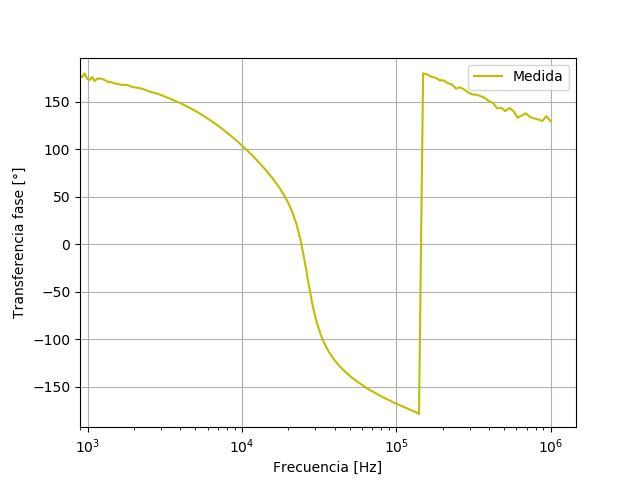
\includegraphics[width=\textwidth]{Imagenes-Ej2/BodeRauchFase.png}
	\label{fig:graph}
\end{figure}

\subsubsection{Etapas.}
Se realizaron 2 etapas, ambas siendo el mismo tipo de celda, pero con distintos parámetros.
\subsubsection{Filtro definitivo.}
%
%\begin{figure}[H]
%	\centering
%	\includegraphics[width=0.4\textwidth]{/ImagenesEjercicio3/Graph.png}
%	\label{fig:graph}
%\end{figure}

\end{document}	
	\newpage	

\section{Aproximacion de Cauer con celda Sedra}
	\documentclass[a4paper]{article}
\usepackage[utf8]{inputenc}
\usepackage[spanish, es-tabla]{babel}

\usepackage{amsmath}
\usepackage{amsfonts}
\usepackage{amssymb}

\usepackage{float}
\usepackage{graphicx}
\usepackage{subcaption}
\captionsetup{compatibility=false}

\usepackage{multirow}
\setlength{\doublerulesep}{\arrayrulewidth}

\usepackage{array}
\newcolumntype{C}[1]{>{\centering\let\newline\\\arraybackslash\hspace{0pt}}m{#1}}

\usepackage[american]{circuitikz}

\usepackage{fancyhdr}

\usepackage{units} 

\pagestyle{fancy}
\fancyhf{}
\lhead{22.01 Teoría de Circuitos}
\rhead{Mechoulam, Lambertucci, Rodriguez, Londero}
\rfoot{Página \thepage}
\begin{document}

\section{Medici\'on corriente de bias y tensi\'on de offset}

\subsection{Introducción}
Las corrientes de \textbf{bias} son las corrientes de polarización de la electrónica dentro de los amplificadores operacionales, en el informe se analizará 2 operacionales, uno con corrientes de bias atribuidas a la corriente de base de un par diferencial de bjt a la entrada del mismo y otro implementado con jfet que si bien teoricamente no deberia tener corriente de gate realmente la tiene.
La tension de offset es la diferencia de potencial que se encuentra a la salida del operacional teniendo una tension nula a la entrada.
Otra corriente de interes es la Corriente de offset.
Con el modelo del Op Amp que tiene en cuenta estos fenomenos se puede definir.\newline
 	
 $I_{offSet} \ = \ |I_b^{-}-I_b^{+}|$\ y \ $I_{Bias}= \frac{I_b^-+I_b^{+}}{2}$
\begin{figure}[htb]	
	\centering
	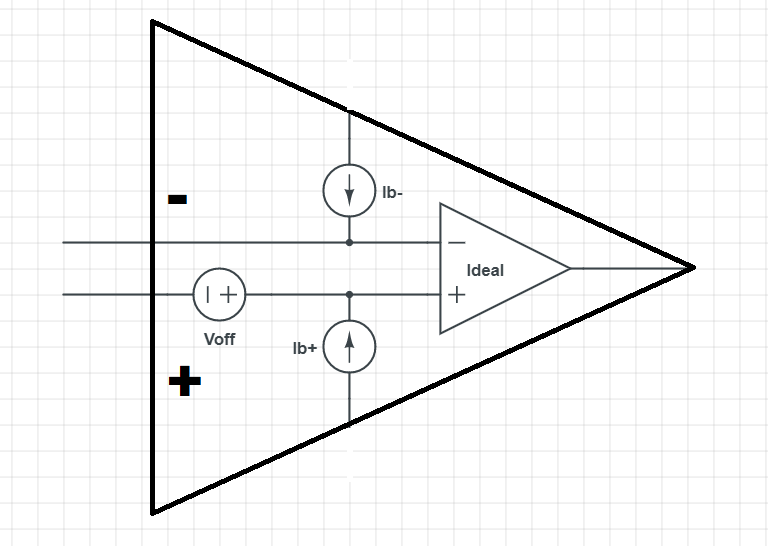
\includegraphics[width=0.7\textwidth]{imagenes/opampReal.PNG}
	\caption{Modelo OpAmp con corriente de bias y tensión de offset.}
	\label{fig:OpampBias}
\end{figure}



Se proporcionó el siguiente circuito para medir las corrientes de bias y la tension de offset.

\begin{figure}[htb]	
	\centering
	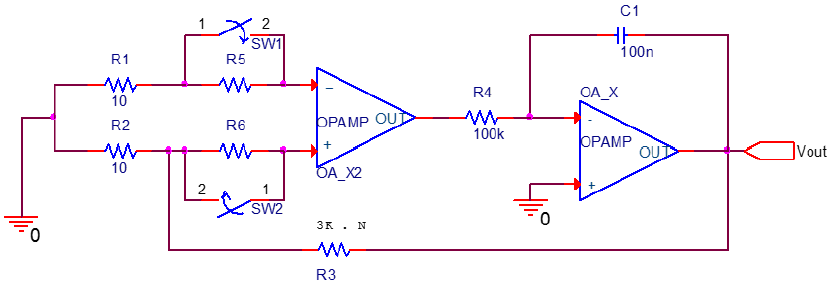
\includegraphics[width=0.7\textwidth]{imagenes/CircMedicion.PNG}
	\caption{Circuito de medición.}
	\label{fig:CircMedicion}
\end{figure}

\subsection{Estabilidad}
Se analizó cada modulo del circuito por separado realizando el diagrama de flujo de señal para el analisis de estabilidad.\\
Se comenzó por la segunda parte dado que es necesario un resultado de esta parte para realizar la primera

\begin{figure}[htb]	
	\centering
	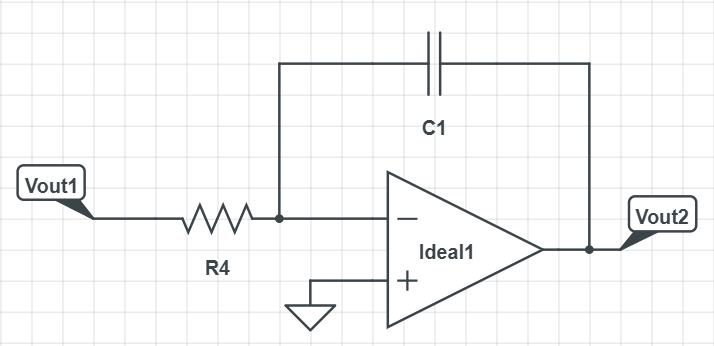
\includegraphics[width=0.7\textwidth]{imagenes/SegundaEtapa.PNG}
	\caption{Segunda Etapa.}
	\label{fig:SegundaEtapa}
\end{figure}
La corriente circulara a travez de la resistencia y el capacitor.\\
\begin{center}
$ \frac{V_{out_1}-V^-}{R_4} = (V^--V_{out_2})\cdot sc$ \\
\end{center}
 Despejando para \ $V^-$ \ se llega a: \\
\begin{center}
$V^- = V_{out_1} \cdot \frac{1}{scR_4+1}+V_{out_2} \cdot \frac{scR_4}{scR_4+1}$\\\end{center}
y utilizando la ecuación del OpAmp:\\
\begin{center}
$V_{out_2}=A_0 \cdot (-V^-)$
\end{center}
Se llega al siguiente diagrama
\begin{figure}[H]	
	\centering
	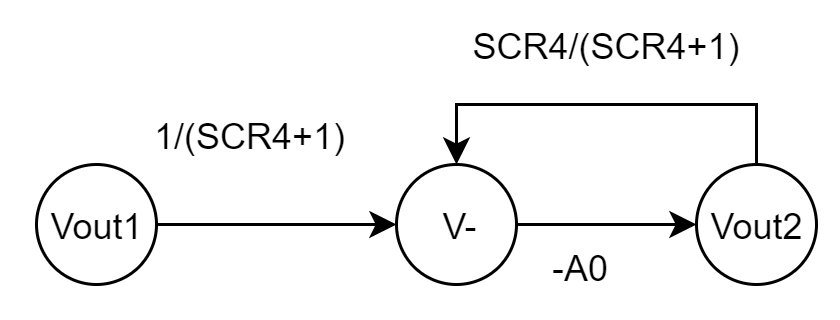
\includegraphics[width=0.7\textwidth]{imagenes/SegundaEtapaDiagrama.PNG}
	\caption{Diagrama de flujo de señal de la segunda etapa.}
	\label{fig:SegundaEtapaDiagrama}
\end{figure}
De aqui se puede apreciar que el circuito es estable dado a que la realimentacion es negativa y por lo tanto estable, si se invitiese la entrada, el circuito pasaria a ser inestable\\
Luego analizando la primer etapa
\begin{figure}[H]	
	\centering
	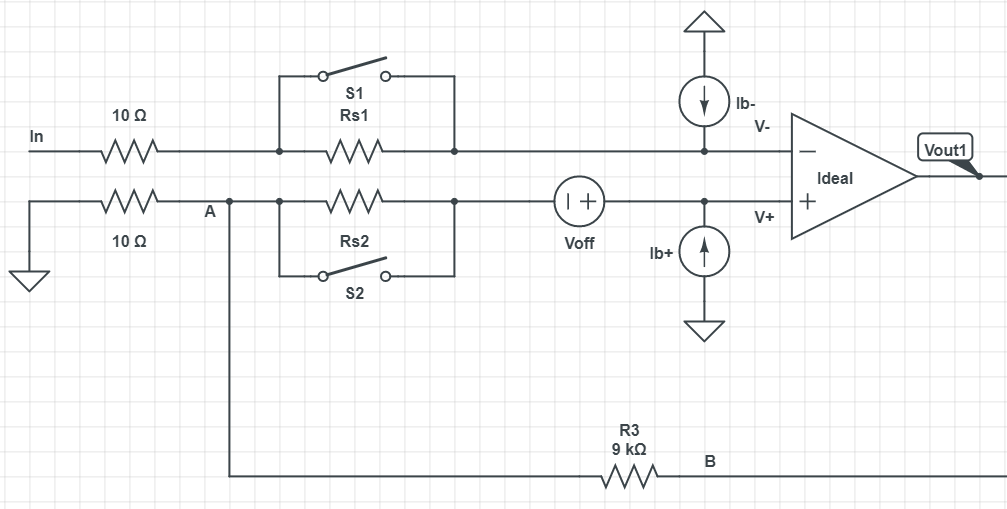
\includegraphics[width=0.7\textwidth]{imagenes/PrimeraEtapa.PNG}
	\caption{Primer Etapa.}
	\label{fig:PrimerEtapa}
\end{figure}
Sabiendo que la tensión en B sera el resultado de la confiugración inversora de la segunda etapa.\\
\begin{center}$V_{out_1}=A_0 \cdot (V^+ - V^-)$\\\end{center}
\begin{center}$V^+= V_{out_1}\cdot \frac{-1}{SCR_4} \cdot \frac{10}{10+R_3} $\\\end{center}
\begin{center}$V^- = V_{in}$\\\end{center}
Se obtiene el diagrama de flujo de señal:
\begin{figure}[H]	
	\centering
	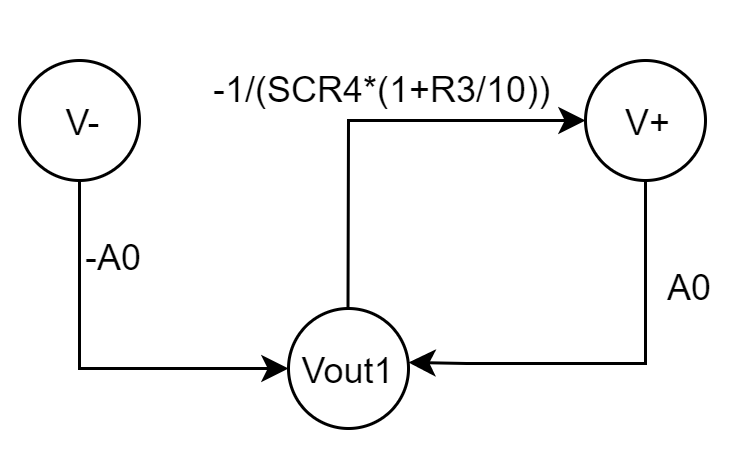
\includegraphics[width=0.7\textwidth]{imagenes/PrimerEtapaDiagrama.PNG}
	\caption{Diagrama de flujo de señal de la primer etapa.}
	\label{fig:PrimerEtapaDiagrama}
\end{figure}
El cual tambien se puede notar que es estable dado a la realimentacion negativa, en caso de permutar las entradas cambiarian los signos de los lazos y seria inestable.
Finalmente si se invierten las entradas de ambas etapas en simultaneo tambien sera inestable dado que la primer etapa todavia estará con una realimentacion positiva.\\
A modo de conclución se llega a que el la única configuración estable es la original, dado que la permutacion de las entradas lleva a situaciones inestables por la realimentacion positiva.
\subsection{Deducción de expresiones para medir.}

Teniendo en cuenta el circuito entero de medicion, las corrientes de bias y la tension de offset se lo puede modelar de la siguiente manera
\begin{figure}[H]	
	\centering
	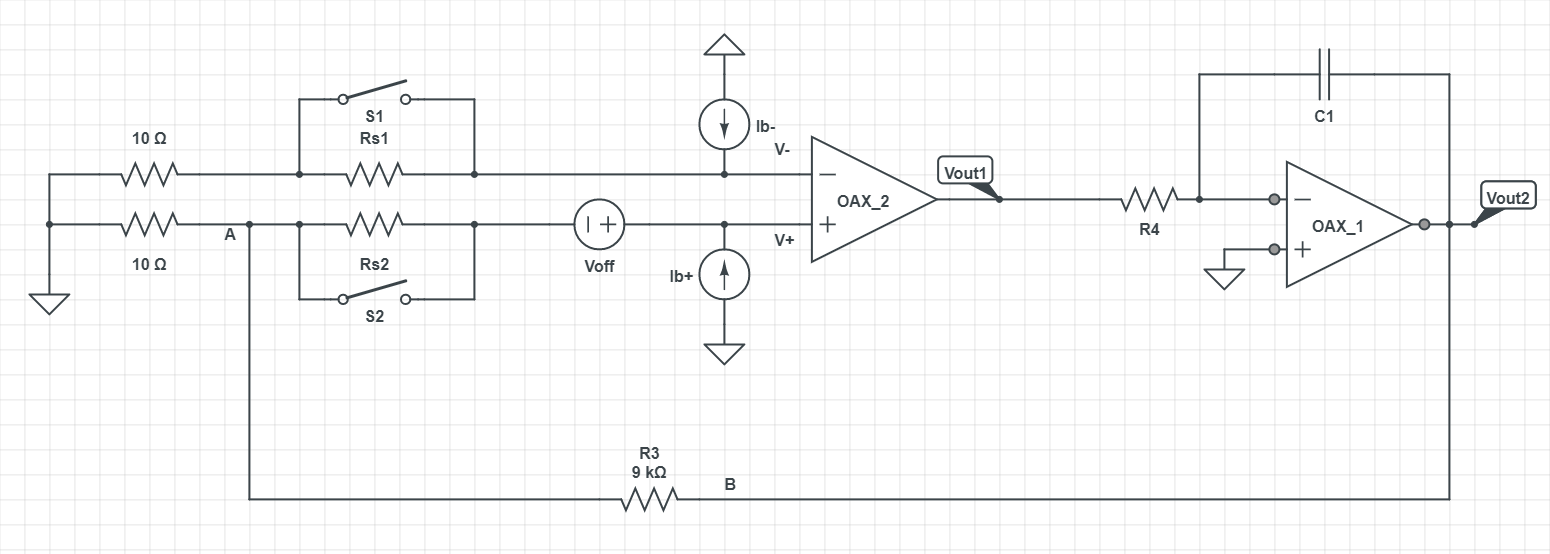
\includegraphics[width=\textwidth]{imagenes/Medicion.PNG}
	\caption{Circuito de medición.}
	\label{fig:Medicion}
\end{figure}
El Opamp a medir será el OAX-2
\begin{center}$V_{out_1}=A_0 \cdot (V^+ - V^-)$\\\end{center}
Dado a que la corriente de bias es unicamente continua para la segunda etapa el opamp es como si estuviese a lazo abierto\\
\begin{center}$V_{out_2}=A_0 \cdot V_{out_1}$\\\end{center}
\begin{center}$V^-=I_b^- \cdot (R_{s2}+10)$\\\end{center}
\begin{center}$V^+=I_b^+ \cdot R_{s1} +V_A+V_{off}$\\\end{center}
\begin{center}$V_A=V_{out_2} \cdot \frac{1}{1+\frac{10}{R_3}}$\\\end{center}
Despejando para $V_{out_2}$ se llega a:
\begin{center}$V_{out_2}=A_0^2  \cdot \frac{I_b^+ \ R_{s1} -I_b^-\cdot (R_{s2}+10)+V_{off}}{1-A_0^2 \cdot \frac{1}{1+\frac{10}{R_3}}}$\\\end{center}
$\lim_{A_0\to\infty} A_0^2  \cdot \frac{I_b^+ \ R_{s1} -I_b^-\cdot (R_{s2}+10)+V_{off}}{1-A_0^2 \cdot \frac{1}{1+\frac{10}{R_3}}}=-(I_b^+ \ R_{s1} -I_b^-\cdot (R_{s2}+10)+V_{off})\cdot \frac{1}{1+\frac{10}{R_3}} $
Luego cambiando de posicion la llave se va apoder medirlos diferentes observavles de interes del circuito.\\
La $V_{off}$ se medirá poniendo en corto $R_{s1}$ y $R_{s2}$ y se despreciará la caida sobre el resistor de 10$\Omega$ dado a su pequeño valor y que la corriente de bias tambien es muy pequeña.\\
\begin{center}$V_{off}=V_{out_2} \cdot \frac{10}{10+R_3} $\end{center}
Ahora que se tiene un valor de $V_{off}$ se  puede poner en corto S1 ó S2 arbitrariamente y se conseguirá una expresión para $ I_b^+ \ o \  I_b^-$ en función de $V_{off} \ y \ V_{out_2}$
Se tuvo en cuenta elegir un valor de resistecia alto para $R_{s1}$ y $R_{s2}$ talque sea mas apreciable la caida de potencial sobre ellas; se eligió 1 Mega dado a que siendo un valor muy grande se podrá despreciar la caida de potencial sobre $R_{s2}$  cuando se mida $I_b^+$.\\
\begin{center}$I_b^+=\frac{V_{out_2} \cdot \frac{10}{10+R_3}-V_{off}}{R_{s1}}$\end{center}
\begin{center}$I_b^-=\frac{V_{out_2} \cdot \frac{10}{10+R_3}-V_{off}}{R_{s2}+10}$\end{center}

\subsection{Ruido Ambiente.}
La segunda etapa si bien está a lazo abierto para las corrientes de bias dado que es de continua se comporta como un filtro para el ruido ambiente que se encuentra a 50Hz,con los valores actuales de resistencia y capacitor atenuará $\approx$ 0.45dB, aumentando el valor del capacitor a 1$\mu F$ sera de  $\approx$ 20dB.
Un problema que se presentaria aplicando un capacitor demasiado chico es que el ruido haría mucho mas dificil las mediciones.
\subsection{Resultados.}
\subsubsection{Mediciones}
Se midio el circuito utilizando osciloscopio y se  obtuvo la siguiente tabla.



\begin{table}[H]
\begin{center}
\begin{tabular}{|c|c|c|c|}
\hline
\multicolumn{4}{|c|}{\textbf{Mediciones}}                                        \\ \hline
\textbf{LF356}        & \multicolumn{3}{c|}{\textbf{Vout}}                       \\ \hline
\textbf{Switches}     & $R_{S1}$ y $ R_{S2} = 0$ & $ R_{S2} = 0$ & $ R_{S1} = 0$ \\ \hline
\textbf{Osciloscopio} & -1.3V                    & -1.4431V      & -1.3903V      \\ \hline
\textbf{TL081}        & \multicolumn{3}{c|}{\textbf{Vout}}                       \\ \hline
\textbf{Switches}     & $R_{S1}$ y $ R_{S2} = 0$ & $ R_{S2} = 0$ & $ R_{S1} = 0$ \\ \hline
\textbf{Osciloscopio} & 0.338V                   & 0.348V        & 0.282V        \\ \hline
\end{tabular}
\end{center}
\end{table}

Si bien estos fueron los resultados finales de la medición, inicialmente se tuvo el inconveniente de que había mucha interferencia de linea y el opamp terminaba saturando dado a la componente no inversora provista por el ruido de linea, el cual invertia el lazo de realimentacion y terminaba oscilando.
Lo cual daba la siguiente señal.
\begin{figure}[H]	
	\centering
	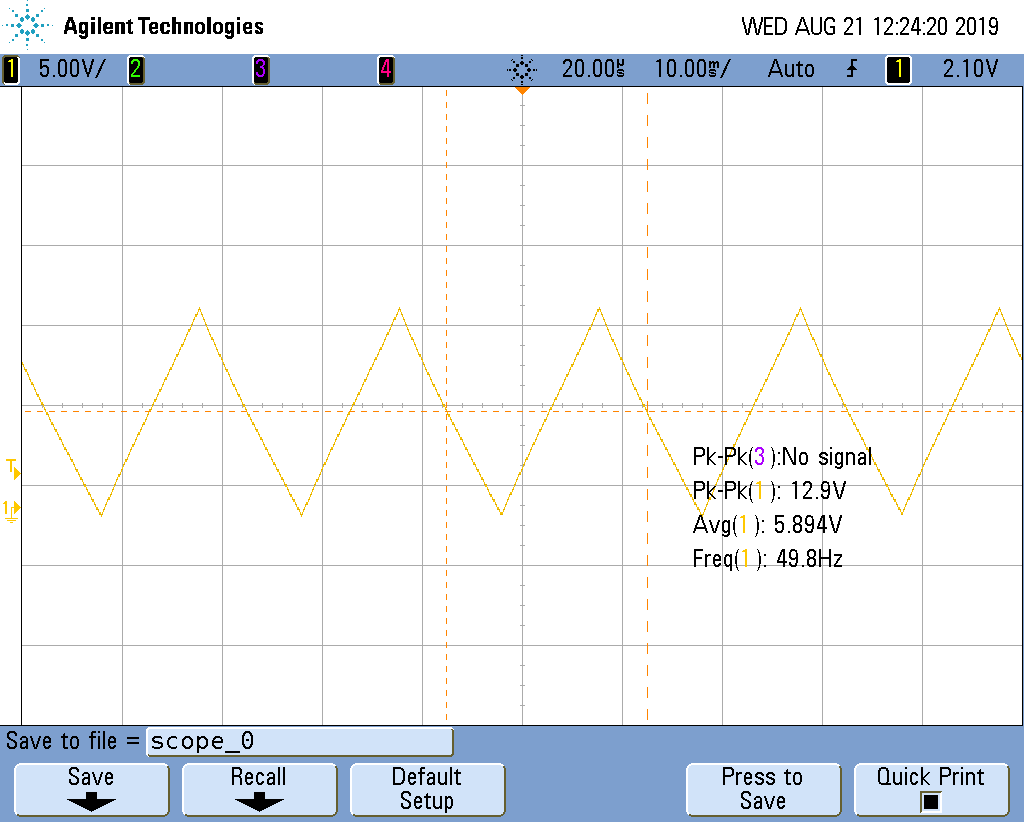
\includegraphics[width=0.5\textwidth]{imagenes/opmpOscilando.png}
	\caption{Circuito Oscilando.}
	\label{fig:oscilando}
\end{figure}
Luego se volvio a medir cambiando el capacitor por uno de 1$\mu F$ 
y  se pudo realizar una medición certera .Obteniendo para los valores de salida para la medición de $I_b^+$ y $I_b^-$. El aumento en el ruido de linea puede deberse a el instrumental que estaba siendo utilizado en el momento en el laboratorio.
Estas fueron las mediciones realizadas previo a el cambio del capacitor:
\begin{figure}[H]
\centering
\begin{minipage}{.5\textwidth}
  \centering
  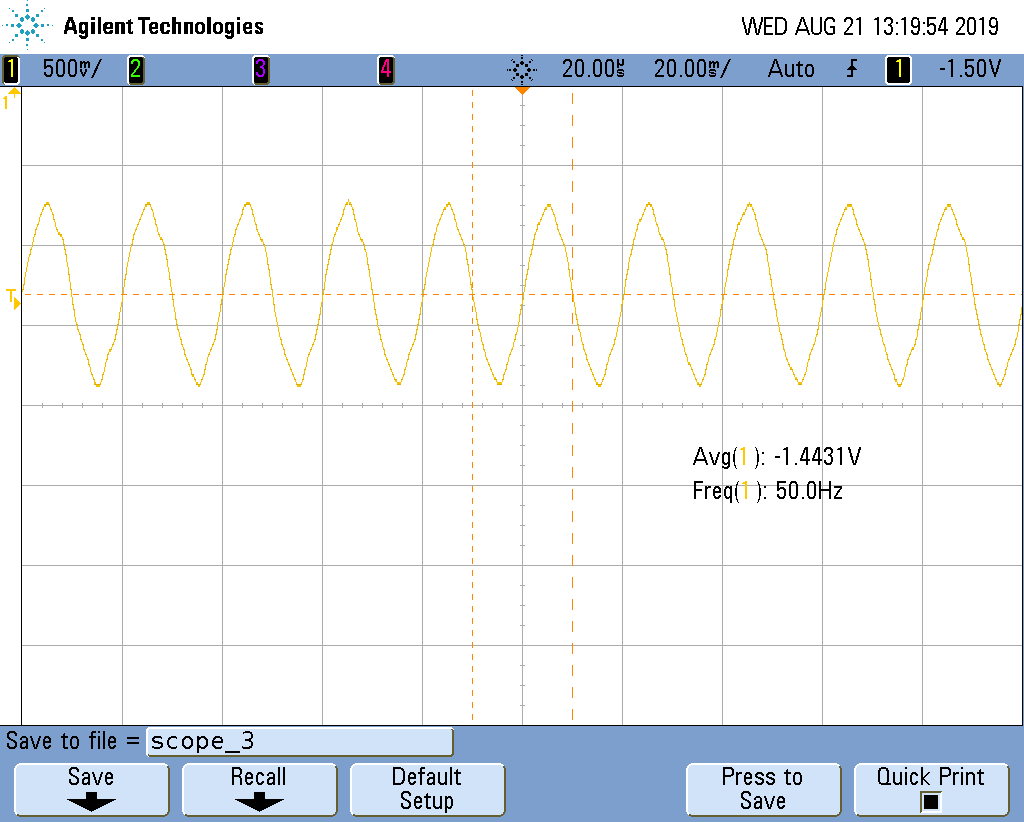
\includegraphics[width=.99\linewidth]{imagenes/IB+.png}
  \captionof{figure}{Medición de Vout para Ib+  LF356}
  \label{fig:ib+}
\end{minipage}%
\begin{minipage}{.5\textwidth}
  \centering
  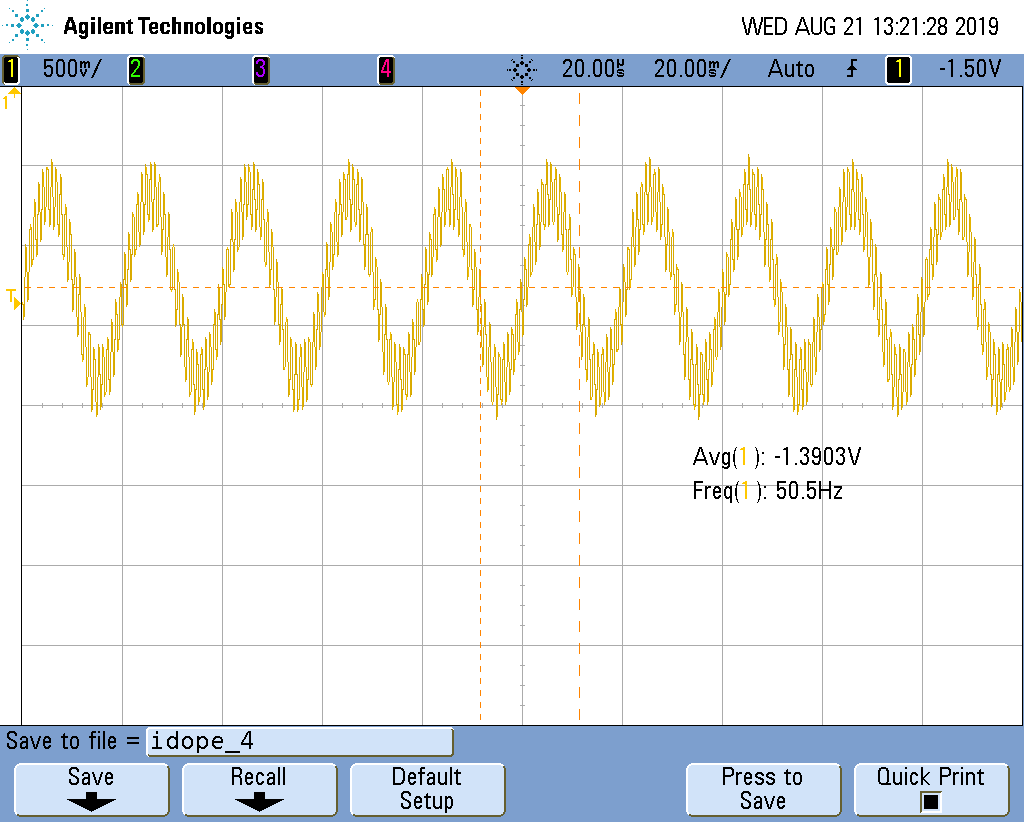
\includegraphics[width=.99\linewidth]{imagenes/IB-.png}
  \captionof{figure}{Medición de Vout para Ib- LF356}
  \label{fig:ib-}
\end{minipage}
\end{figure}

\begin{figure}[H]
\centering
\begin{minipage}{.5\textwidth}
  \centering
  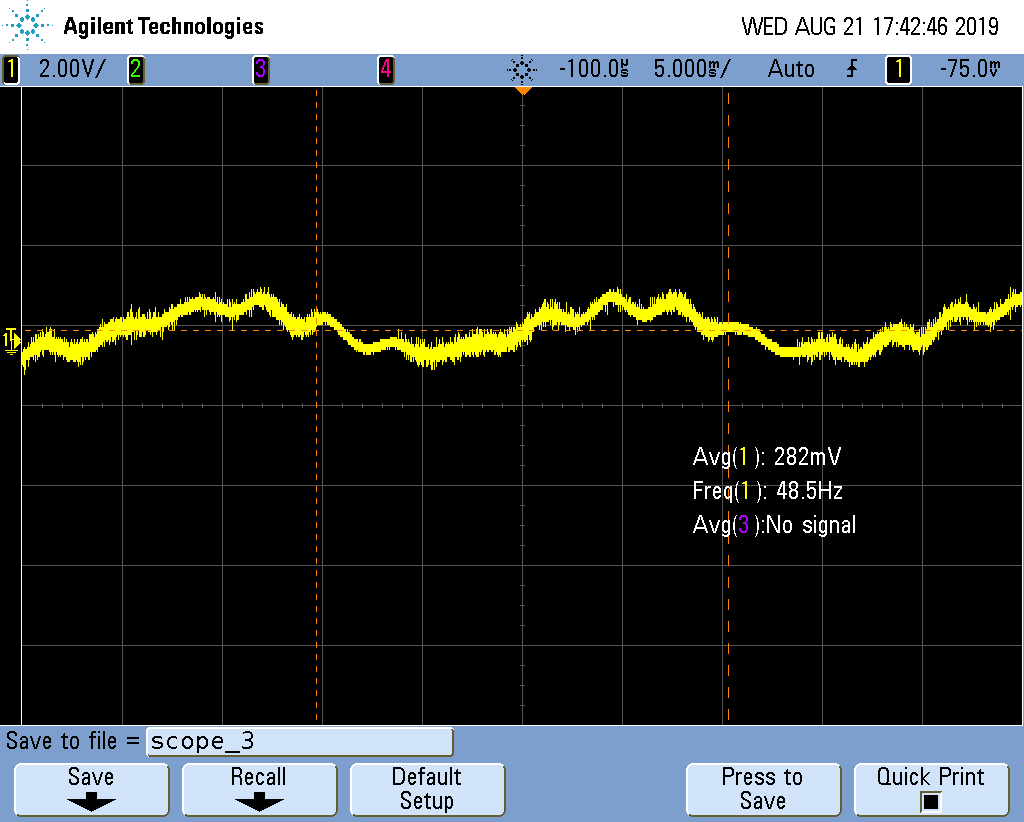
\includegraphics[width=.99\linewidth]{imagenes/RS2CORTO.png}
  \captionof{figure}{Medición de Vout para Ib+  TL081}
  \label{fig:ib+TL}
\end{minipage}%
\begin{minipage}{.5\textwidth}
  \centering
  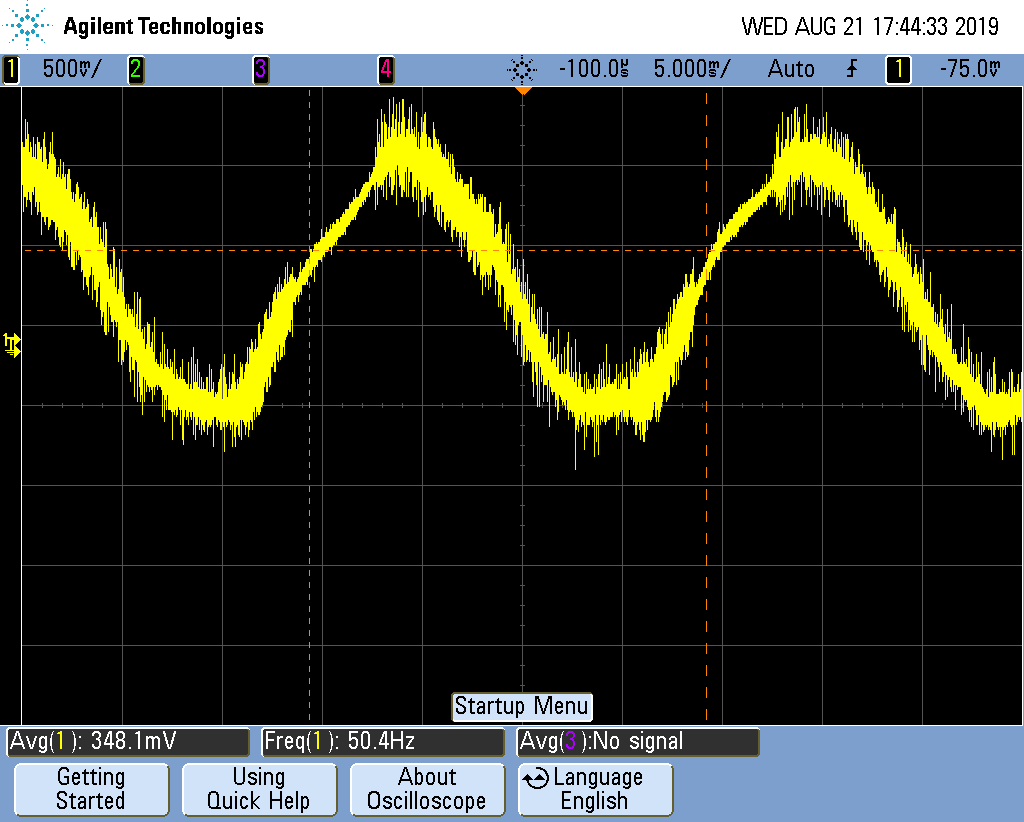
\includegraphics[width=.99\linewidth]{imagenes/RS1CORTO.png}
  \captionof{figure}{Medición de Vout para Ib- TL081}
  \label{fig:ib-TL}
\end{minipage}
\end{figure}
Luego del cambio del capacitor  se obtuvieron las siguientes mediciones, las cuales son en su mayoria libres de ruido.

\begin{figure}[H]
\centering
\begin{minipage}{.5\textwidth}
  \centering
  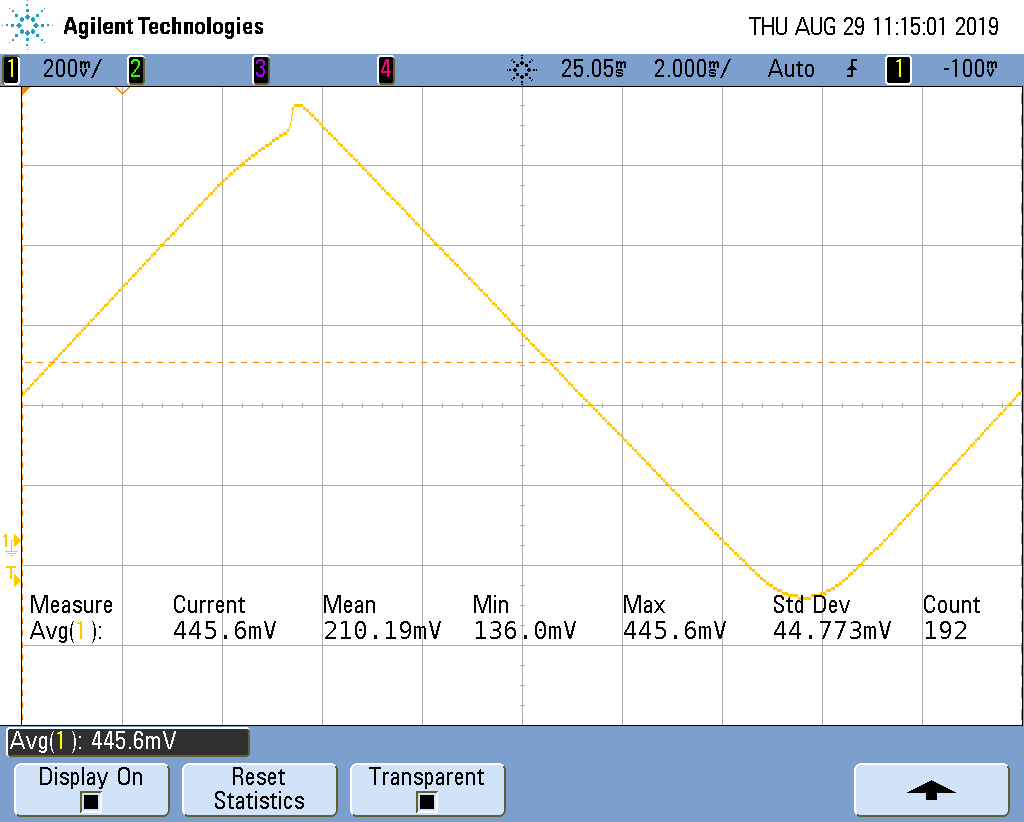
\includegraphics[width=.99\linewidth]{imagenes/RS2CORTOLF356capa.png}
  \captionof{figure}{Medición de Vout para Ib+  LF356 con capacitor}
  \label{fig:ib+}
\end{minipage}%
\begin{minipage}{.5\textwidth}
  \centering
  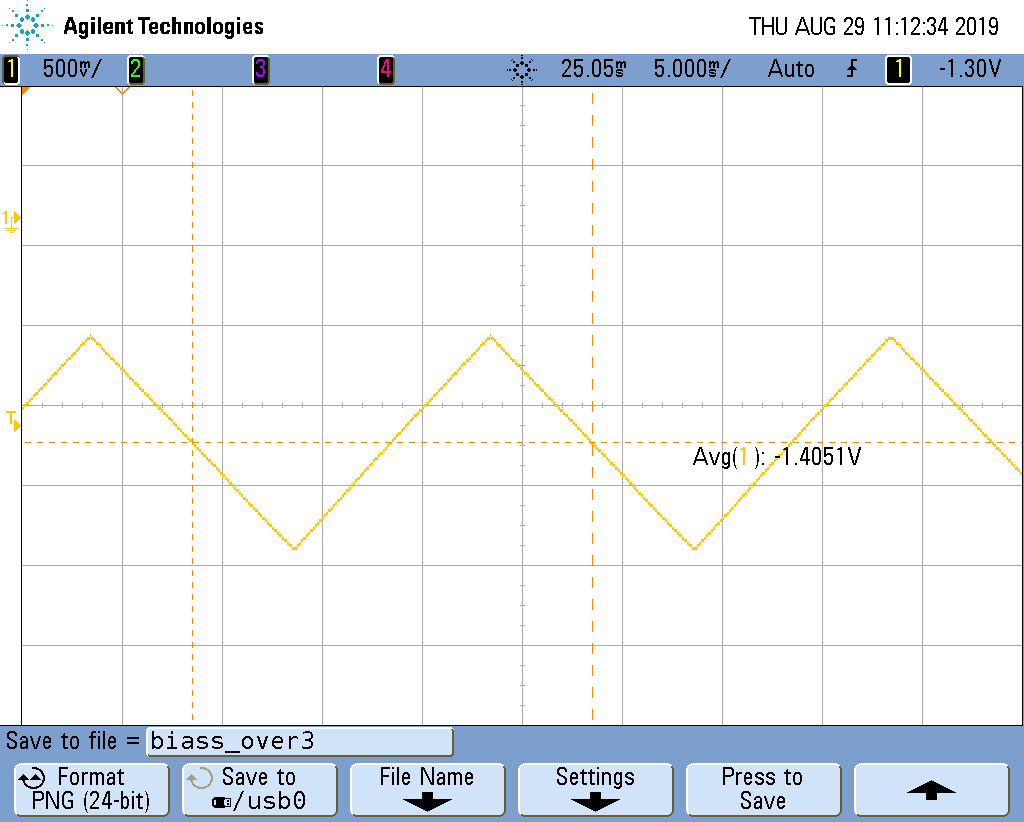
\includegraphics[width=.99\linewidth]{imagenes/RS1CORTOLF356capa.png}
  \captionof{figure}{Medición de Vout para Ib- LF356 con capacitor}
  \label{fig:ib-}
\end{minipage}
\end{figure}

\begin{figure}[H]
\centering
\begin{minipage}{.5\textwidth}
  \centering
  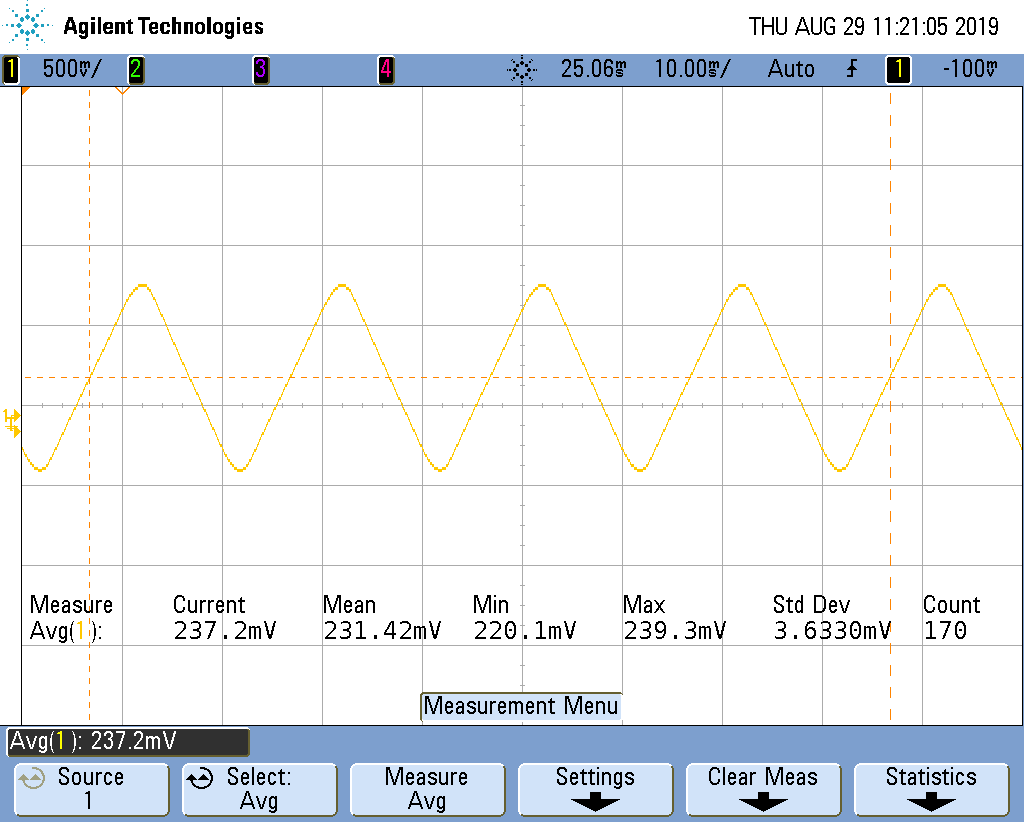
\includegraphics[width=.99\linewidth]{imagenes/RS2CORTOTL081.png}
  \captionof{figure}{Medición de Vout para Ib+  TL081 con capacitor}
  \label{fig:ib+TL}
\end{minipage}%
\begin{minipage}{.5\textwidth}
  \centering
  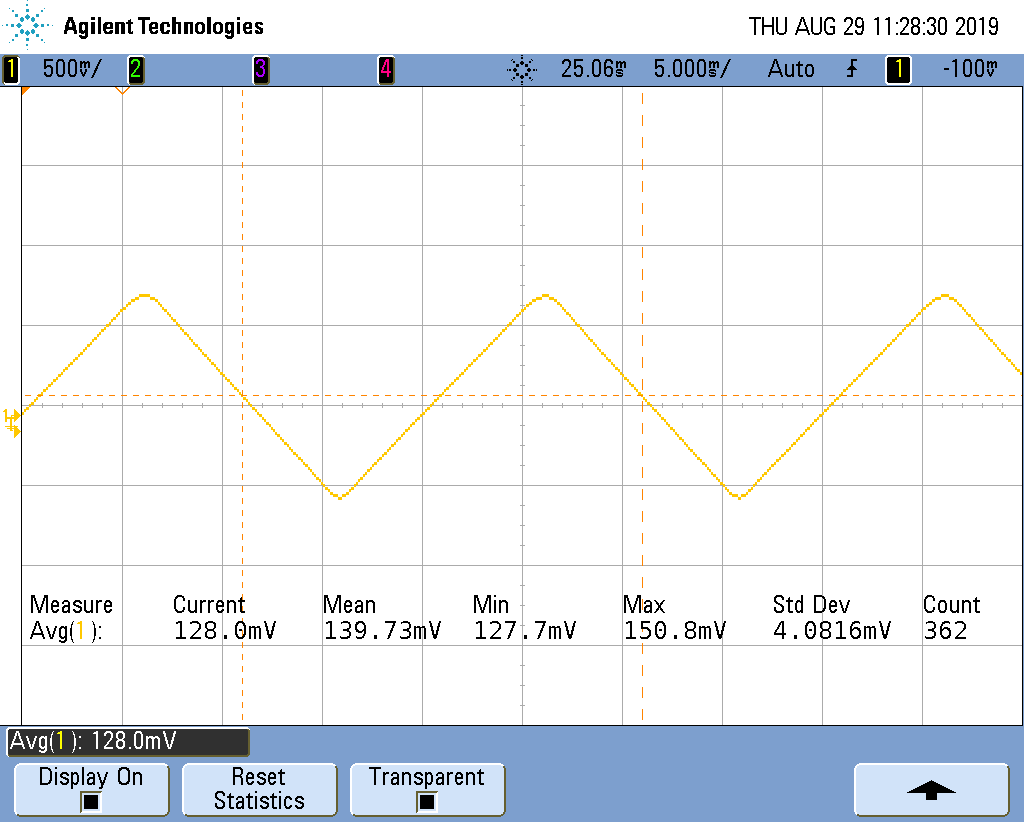
\includegraphics[width=.99\linewidth]{imagenes/RS1CORTOTL081.png}
  \captionof{figure}{Medición de Vout para Ib- TL081 con capacitor}
  \label{fig:ib-TL}
\end{minipage}
\end{figure}
Obteniendo con el nuevo capacitor las siguientes mediciones:

\begin{table}[H]
\begin{center}
\begin{tabular}{|c|c|c|c|}
\hline
\multicolumn{4}{|c|}{\textbf{Mediciones con capacitor}}                                        \\ \hline
\textbf{LF356}        & \multicolumn{3}{c|}{\textbf{Vout}}                       \\ \hline
\textbf{Switches}     & $R_{S1}$ y $ R_{S2} = 0$ & $ R_{S2} = 0$ & $ R_{S1} = 0$ \\ \hline
\textbf{Osciloscopio} & -1.36V                    & 0.208V      & -1.47V      \\ \hline
\textbf{TL081}        & \multicolumn{3}{c|}{\textbf{Vout}}                       \\ \hline
\textbf{Switches}     & $R_{S1}$ y $ R_{S2} = 0$ & $ R_{S2} = 0$ & $ R_{S1} = 0$ \\ \hline
\textbf{Osciloscopio} & 0.332V                   & 0.203V        & 0.138V        \\ \hline
\end{tabular}
\end{center}
\end{table}

\subsubsection{Analisis de resultados.}
A partir de los valores obtenidos en la   \ref{tab:vout} se pueden calcular las corrientes de offset y bias, al igual que la tension de offset previo al cambio de capacitor:
\begin{table}[H]
\begin{center}
\begin{tabular}{|c|c|c|c|c|c|}
\hline
\textbf{LF356} & \textbf{$V_{Offset}$} & \textbf{$I_b^+$} & \textbf{$I_b^-$} & \textbf{$I_{bias}$} & \textbf{$I_{Offset}$} \\ \hline
               & -1.44mV                & -159pA           & -100pA           & -130pA               & 58.6pA                 \\ \hline
\textbf{TL081} & \textbf{$V_{Offset}$} & \textbf{$I_b^+$} & \textbf{$I_b^-$} & \textbf{$I_{bias}$} & \textbf{$I_{Offset}$} \\ \hline
\textbf{}      & 0.375mV                & 11.1pA           & 62pA             & 25.5pA               & 73.3pA                 \\ \hline
\end{tabular}
\end{center}
\end{table}
Luego con el capacitor cambiado:
\begin{table}[H]
\begin{center}
\begin{tabular}{|c|c|c|c|c|c|}
\hline
\textbf{LF356 con capacitor} & \textbf{$V_{Offset}$} & \textbf{$I_b^+$} & \textbf{$I_b^-$} & \textbf{$I_{bias}$} & \textbf{$I_{Offset}$} \\ \hline
               & -1.51mV                & -92pA           & -33.6pA           & -62.9pA               & 58.6pA                 \\ \hline
\textbf{TL081 con capacitor} & \textbf{$V_{Offset}$} & \textbf{$I_b^+$} & \textbf{$I_b^-$} & \textbf{$I_{bias}$} & \textbf{$I_{Offset}$} \\ \hline
\textbf{}      & 0.368mV                & 143pA           & 215pA             & 179pA               & 71.9pA                 \\ \hline
\end{tabular}
\end{center}
\end{table}
Luego comparandola con la siguiente tabla de valores proporcionada por el fabricante:
\begin{table}[H]
\begin{center}
\begin{tabular}{|c|c|c|c|c|c|}
\hline
\multicolumn{6}{|c|}{\textbf{Datos fabricante LF356}}                                                                                     \\ \hline
\multicolumn{3}{|c|}{\textbf{Máximo}}                               & \multicolumn{3}{c|}{\textbf{Típico}}                                \\ \hline
\textbf{$V_{Offset}$} & \textbf{$I_{bias}$} & \textbf{$I_{offset}$} & \textbf{$V_{Offset}$} & \textbf{$I_{bias}$} & \textbf{$I_{offset}$} \\ \hline
10mV                  & 200pA               & 50pA                  & 3mV                   & 20pA                & 3pA                   \\ \hline
\multicolumn{6}{|c|}{\textbf{Datos fabricante TL081}}                                                                                     \\ \hline
\multicolumn{3}{|c|}{\textbf{Máximo}}                               & \multicolumn{3}{c|}{\textbf{Típico}}                                \\ \hline
\textbf{$V_{Offset}$} & \textbf{$I_{bias}$} & \textbf{$I_{offset}$} & \textbf{$V_{Offset}$} & \textbf{$I_{bias}$} & \textbf{$I_{offset}$} \\ \hline
10mV                  & 400pA               & 100pA                 & 3mV                   & 20pA                & 5pA                   \\ \hline
\end{tabular}
\end{center}
\end{table}
Se puede observar que la mayoria de los valores se encuentran dentro de las tolerancias admitidas por el fabricante, el desvio en la corriente de Offset es atribuido a los componentes que su valor no es preciso, que no se tuvo en cuenta a la punta del osciloscopio en el modelo.
Tambien se le atribuye la diferencia en valores en particualr en la corriente  de bias del TL081 entre las medidciones sin cambiar el capacitor y las hechas con el capacitor a el ruido que se tenia en el sistema.
\subsection{Compensacion de tension de offset y corrientes de bias.}
\subsubsection{Compensación Bias}
Para la compensacion de corriente de bias lo que se desea es hacer que la diferencia entre $I_b^+$ y $I_b^-$ sea $\approx$ 0
Un ejemplo de esto es tomar un Op Amp en configuración inversora  de las sigueintes caracteristicas:
\begin{figure}[H]	
	\centering
	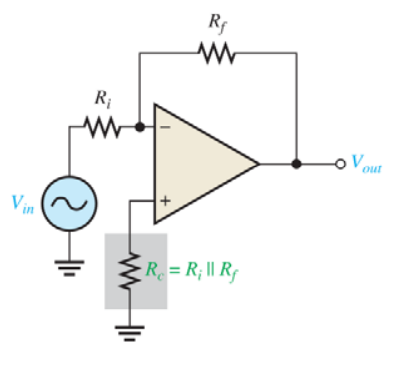
\includegraphics[width=0.5\textwidth]{imagenes/CompensacionBias.PNG}
	\caption{Circuito inversor para la compensacion de BIAS.}
	\label{fig:CompensacionBias}
\end{figure}
Asumiendo ya compensada la tension de offset se procede a la deducción de el valor de Rc para minimizar las corrientes de bias.
\begin{center}$V_{out}=A_0 \cdot (V^+ - V^-)$\\\end{center}
\begin{center}$V^+=-I_b^+ \cdot R_c$\\\end{center}
\begin{center}$\frac{V_{in}-V^-}{R_i}=\frac{V^- - V_{out}}{R_f} -I_b^-$\\\end{center}
Despejando para $V_{out}$ queda:
\begin{center}$V_{out}=V_{in}\cdot -\frac{R_f}{R_i}+I_b^+ R_f-I_b^- R_c \cdot \frac{R_i+R_f}{R_i R_f}\cdot R_f $\\\end{center}
Teniendo un valor de $R_c$= $R_i//R_f$ se deberian anular o atenuar significativamente las corrientes de bias.
\subsubsection{Compensación Tension de Offset}
Para la compensación de la tension de offset hay varias alternativas. En el caso de los Opamps que fueron usados en este informe cuentan con unos pines para configurar la tension de offset(1 y 5), la forma que se va a desarrollar es un circuito externo que funcione en configuracion inversora.
El circuito a implementar es el siguiente:
\begin{figure}[H]	
	\centering
	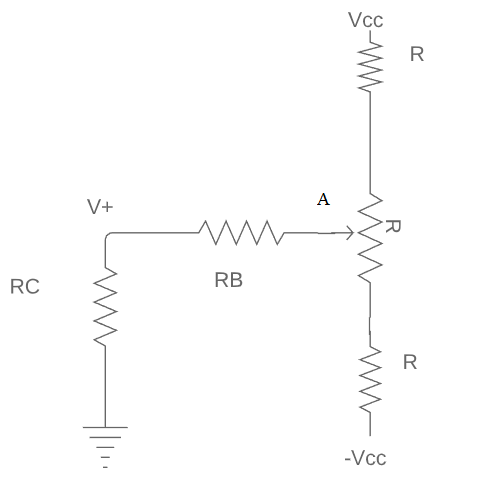
\includegraphics[width=0.5\textwidth]{imagenes/CompensacionOff.PNG}
	\caption{Circuito para la compensacion de Tension de Offset.}
	\label{fig:CompensacionOff}
\end{figure}
El potenciometro sera utilizado para variar la tension que se le agrega a $V^+$ a travez del divisor resistivo conformado por $R_C$ y $R_B$ donde Rc podria ser una resistencia para compensar el BIAS. RB debe ser un valor por lo menos 10 veces superior a RC dado que la tension que se quiere corregir es pequeña. el propósito de las 2 resistencias 'R' es aumentar la sensibilidad para elegir la tensión. El valor del potenciometro deberia ser un orden de magnitud menor que $R_B $

\begin{align}
V_{Off}=V^+ = V_A \cdot \frac{R_c}{R_c+R_b}  
\end{align}
\begin{align}
V_A =V_{Off} \cdot \frac{R_c+R_B}{R_c}
\end{align}
A partir del valor de $V_A$ se puede definir un valor de R
\end{document}
	
	\newpage	
	
\end{document}